\chapter{Computational Models for Cardiac Diseases}
\label{chap:cardiac-diseases}

\section{Introduction}
\label{sec:introduction-17}

The normal function of the heart relies on the coordinated propagation of the
action potential (AP), the rhythmic electrical stimulus that triggers the
contraction of the cells. During an action potential (AP), the membrane
potential first depolarize and the repolarize under the dynamic changes of ionic
concentration. While depolarization is a robust process, repolarization is
fragile \citep{tomaselli1994}.
\begin{itemize}
\item Depolarization is generated by 
  \begin{enumerate}
    \item large ($\sim$ 100-fold) increase
  in membrane conductance as the large population of $\na$ channels
  are activated. When it passes the threshold, it's almost impossible to
  stop it from running its full course.
  
    \item Some speculated that the reverse NCX can also trigger the
  depolarization where about 20\%  of NCX resides on the Z-lines.
  \end{enumerate}
  
\item Repolarization, however, is brought about by very tiny
  current. As the fast depolarization phase is complete, the net
  membrane conductance actually falls well below its resting
  value~\cite{weidmann1951}. This is opposite to the AP in nerve
  cell~\citep{cole1939}.
\end{itemize}

The conduction velicity (CV) and action potential duration (APD) depend on
one or more previous diastolic or interbeat intervals. This dependence, called
{\bf restitution}, is considered as an important determinant of the stability of
conduction and is involved in arrhythmias genesis. Many experiments showed
at high frequency, EAD or DAD can be developed
(Sect.\ref{sec:afterdepolarization}). The representation between the interval
between two consecutive beats (ms) and the conduction velocity (cm/s) is known
as the {\bf restitution curve} (or restitution function),
Fig.\ref{fig:restitution_curve}. So, the CV and APD are important parameters
governing arrhythmogenesis. A major factor that affect to CV is conduction
block, at which cells along the conduction pathway cannot trigger an AP.
This can be the result from a reduction of inward membrane currents, a reduction
of gap junctional couling and from tissue inhomogeneities. Also, another major
factor is the spontaneous AP due to the abnormal calcium level and stochastic
chanel behavior. It's thus very important to have a whole-cell model that
incorporate the stochastic gating of ionic channels. As RyR channels are
believed to be a potential drug target, models incorporate stochastic gating of
RyR are considered having good prediction capability.


\begin{figure}[hbt]
  \centerline{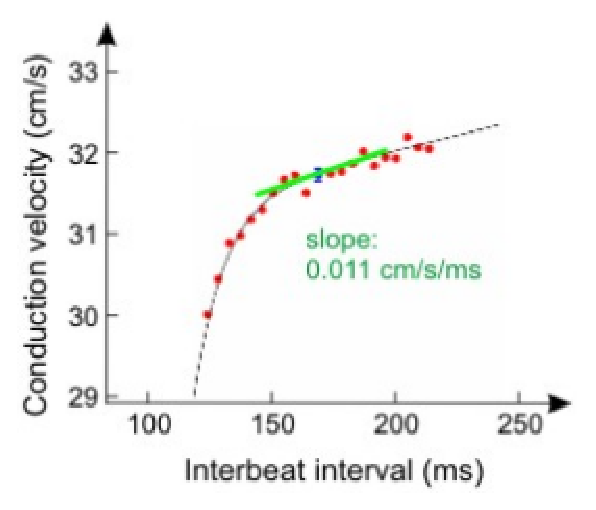
\includegraphics[height=5cm,
    angle=0]{./images/restitution_curve.eps}}
  \caption{Restitution curve
  \footnote{\url{http://www.physio.unibe.ch/~kucera/group/projects.aspx}}}
  \label{fig:restitution_curve}
\end{figure}


\begin{figure}[hbtp]
  \centerline{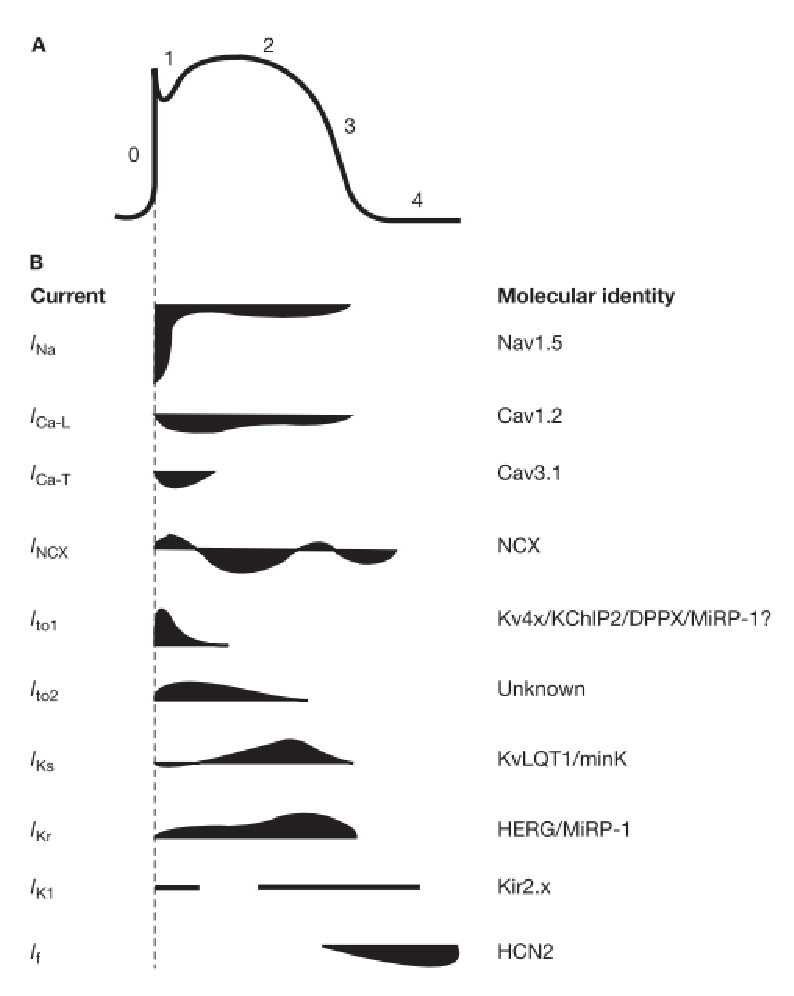
\includegraphics[height=10cm,
    angle=0]{./images/ion_channel_roles.eps}}
  \caption{Roles of ion channels at different phases of AP \citep{nass2008}}
  \label{fig:ion_channel_roles_AP}
\end{figure}

The long APD in cardiac cell has its own purpose,
Fig.\ref{fig:ion_channel_roles_AP}. At rest, transient outward current $I_{K1}$
is on to keep the membrane at very negative potential.
During depolarization, $I_{K1}$ is rapidly switched off; while other currents
take time to activate and to cause repolarization. The mechanism of quickly
turning off $I_{K1}$ is to save energy, as a large amount of ATP is used for
extruding $\Ca$ from the cytosol during dyastolic. At the cellular level, a
modification in cardiac AP can lead to fatal condition. When an AP is
interfered, the modified AP may be followed by one or many oscillations, known
as EAD (Sect.~\ref{sec:early-afterd-ead}).
An example is that~\citep{noble2008}:
\begin{itemize}
\item A 65\% block of $I_{Kr}$ can prevent the smooth repolarization
  and cause EAD.
\item However, combining 65\% block of $I_{Kr}$ with 20\% block of
  $I_\CaL$ can recover the AP to normal. A drug BRL-32872 can do
  this~\citep{bril1995}. 
\end{itemize}

Currently, biological markers to give early warning of possible cardiac problems
are QT interval (Sect.~\ref{sec:long-qt-syndrome}), which are unreliable. Some
drugs cause arrhythmias without prolonging QT and some drugs that prolong QT but
don't cause arrhythmias. hERG is a protein that form the main component of
$I_{Kr}$ that explains one type of long QT syndrome. Some drugs that target hERG
doesn't cause arrhythmias.

Among ion channels, $\Na$ and $\Ca$ channels are the most widely used target to
drug development. $\Na$ channels play an important role to the onset of an AP
(with fast conduction 0.3-3.0 ms). So, $\Na$ channels have been found related to
a number of arrhythmias in ventricular: tachyarrhythmias, ectopic activity, and
possibly in ischemia as  inhibited fast responses.  $\Ca$ channels has a slower
conduction (0.01-0.10 ms), that may cause reentry, a role in early ischemic or
reperfusion arrhythmias.  

In real life, the situation is more complicated. Many factors can interact with
the drugs to make the problem worse, e.g. genetic disease (e.g. mutation in
$\Na$, $\Ca$ ionic channels or RyR (CPVT (Sect.~\ref{sec:cpvt})). The
heterogeneity in ion channels distribution, crosstalk between individual ion
channels, and the complex remodelling in the context of ventricular dysfunction
(e.g. T-tubule remodelling with z-line disruption or reorganization). The
limited understanding of all of these phenomena at the cellular level has not
allow us to understand the proarrhythmic tendency of some of these drugs.
Nevertheless, using a proper computational model can help saving a lot of money
and efforts in drug development.

Computational models of the hearts probably have become the most detailed cell
models so far~\citep{noble2008}. The details of these models will be
discussed in coming chapters. In addition, there have been a number of efforts
to create a general framework for modeling at cellular and tissue level
\begin{enumerate}
\item CellML (\url{http://www.cellml.org})
\item COR (\url{http://cor.physiol.ox.ac.uk})
\item Physiome Project
\end{enumerate}
In this chapter, we will focus on introducing different types of pathological
conditions, and mathematical models that were designed with the goal to provide
some insights into the mechanism of the diseases.



\section{EAD: Zeng-Rudy (1995)}
\label{sec:ead:-zeng-rudy}

~\citep{zeng1995} derived a model based on LR-2 model,
Fig.\ref{fig:Zeng_LR2_1995}  (Sect.~\ref{sec:luo-rudy-phase-2}). Here, all CaRUs
are lumped into a single one. There are also some modifications to better fit
the experimental data
\begin{enumerate}
\item SR $\Ca$ start to release after a delay of 3-9ms. After this,
  time to peak of $[\Ca]_i$ transient is adjusted from 10ms to 15ms,
  by increasing  the activation and inactivation time constant from 2
  to 3.5ms.
\item Peak $[\Ca]_i$ transient 1.0$\mu$M is reached when maximal rate
  constant of calcium release from JSR is adjusted from 60 to
  38ms$^{-1}$. 
\end{enumerate}

\begin{figure}[hbt]
  \centerline{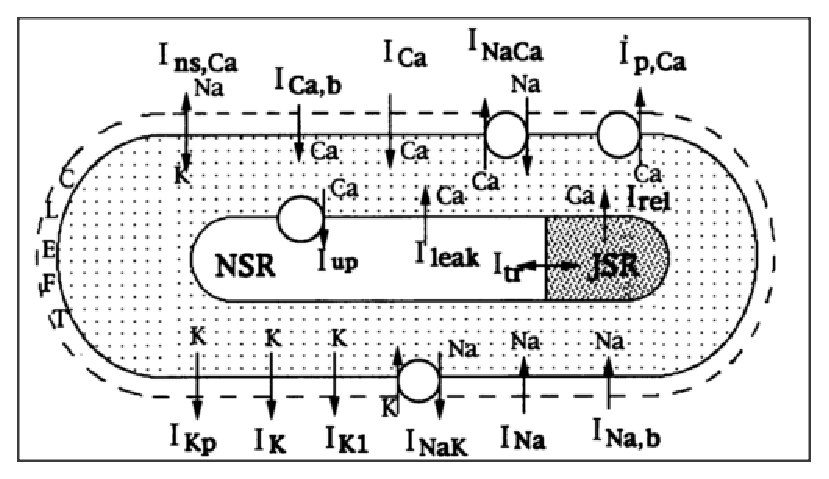
\includegraphics[height=5cm,
    angle=0]{./images/Zeng_LR2.eps}}
  \caption{LR-2 single ventricular cell model }
\label{fig:Zeng_LR2_1995}
\end{figure}


To account for fast pacing, an extracellular region called {\bf cleft}
is added to model the possibility of ion accumulation in the
cleft. The ion concentration change in the cleft is the balance of 2
processes: transmembrane ionic currents and diffusion between the
cleft and the bulk medium with diffusion time
1000ms~\citep{rasmusson1990mme} (Sect.~\ref{sec:rasmusson-et-al}). 

\subsection{Cesium}
\label{sec:cesium}

Cesium is known to depolarize the membrane potential, flatten the
plateau of AP and cause EAD~\citep{isenberg1976}. Low concentration of
Cesium can block the channels; yet high concentration reduce the
$I_\k, I_{K1}$ currents. The effect of reducing is both
$V_m$-dependent and concentration dependent. So, the authors
introduced a scaling factor $\delta_\Cs$.
\begin{equation}
  \label{eq:1459}
  \delta_\Cs = \frac{1}{1+ \exp\left(\frac{V_m-V_{1/2}}{K_\Cs}\right)}
\end{equation}
with $K_\Cs=-16$mV, $V_{1/2}=-95$ (when $[\Cs]=5$mM) and
$V_{1/2}=-40$mV (when $[\Cs]=10$mM). 

\subsection{Isoproterenol}
\label{sec:isoproterenol}

Isoproterenol (ISO) is a $\beta$-adrenergic agonist, which is known to
increase heart rate and enhance contraction. 

ISO increases occurence of spontaneous SR $\Ca release$
as it reduces the threshold for store-overload-induced $\Ca$ release (SOICR)
\citep{Jiang2004}.

\section{Crampin-Smith (2006) - acidosis (cardiac ventricular)}
\label{sec:crampin-smith_06}

\citep{crampin2006, crampin2006am} 

\section{T-tubule remodelling}
\label{sec:T-tubule_remodelling}

Transver tubule (T-tubule) system is a well-organized transervesal invagination
of the surface sarcolemmas into the inner side of the cell that occurs at the
Z-line regions, with pretty much regular spacing ($\approx 2\mum$). It's widely
accepted that this highly organized structure of the T-tubule system is
essential for rapid electrical excitation, initiation and synchronous triggering
of SR calcium releases as many of the proteins involving in EC coupling appear
to concentrate at the T-tubules.

\begin{framed}
At early stage of cell development (neonatal hearts), there is little evidence
of T-tubule development \citep{brette2003}.

T-tubules occur predominantly in ventricular myocytes; while in atrial,
pacemaking and conducting tissues, they are far less developed
\citep{ayettey1978}. Apart from its transversal direction, T-tubules are also
found with longitudinal directions \citep{13}. In addition, only 60\% are found
near the Z-line, with 40\% occurs between the Z-lines \citep{brette2003}. 

The majority of the T-tubule has the diameter in the range 200-300 nm, though
the individual one can vary from 20 to 450nm. The diffusion of calcium from
extracellular calcium into the T-tubule in 3-16 $\mum/s$ \citep{blatter1998}. 
So, the solution change in the T-tubule is delayed by upto 2.3 second.
\end{framed}

In heart failure (HF) condition, which is characterized by a reduction in the
contractile function and dyssynchornous in SR $\Ca$ release, there are several
changes to the cell: (1) reduced SR $\Ca$ leak, (2) RyR hyperphosphorylation,
(3) change in APD \citep{7-10}, (4) a reduction in T-tubule structure
\citep{11-16}. Artificially detubulated myocytes \citep{17-18} also give some
information to.  T-tubule power (TT$_\text{power}$) index is a quantitative
method to determined the frequency of T-tubule structure based on spectrum
analysis (0.5$\mum^{-1}$ corresponds to spatial distance of 2$\mum$ between
T-tubule along x-direction). The sparse irregular T-tubule would not give a
dominant peak in fast-Fourier transform (FFT) power spectrum. Early studies on
T-tubule structure are based on electron microscopy \citep{23,24,25}. Recently,
confocal microscopy was used to investigate T-tubule structure \citep{11-15,
26-33}.

\textcolor{red}{The question is T-tubule remodelling is the early stage or late
event in HF?}. \citep{wei2010} suggested it's the critical early event for the
transition from compensated hypertrophy to decompensated HF,
Fig.\ref{fig:Ttubule_remodelingWei2010}. T-tubule remodelling was already found
at compensated hypertrophy stage, i.e.
discrete local loss and global T-tubule structural reorganization. At advaned
HF, there is massive T-tubule disruption (86\%).
Importantly, there is a significant difference in T-tubule remodelling effect
between LV and RV (right-ventricle) based on TT$_\text{power}$ in hypertrophy
and early HF. The loss of T-tubule is strongly correlated with the loss of JP-2
expression.

\begin{figure}[hbt]
  \centerline{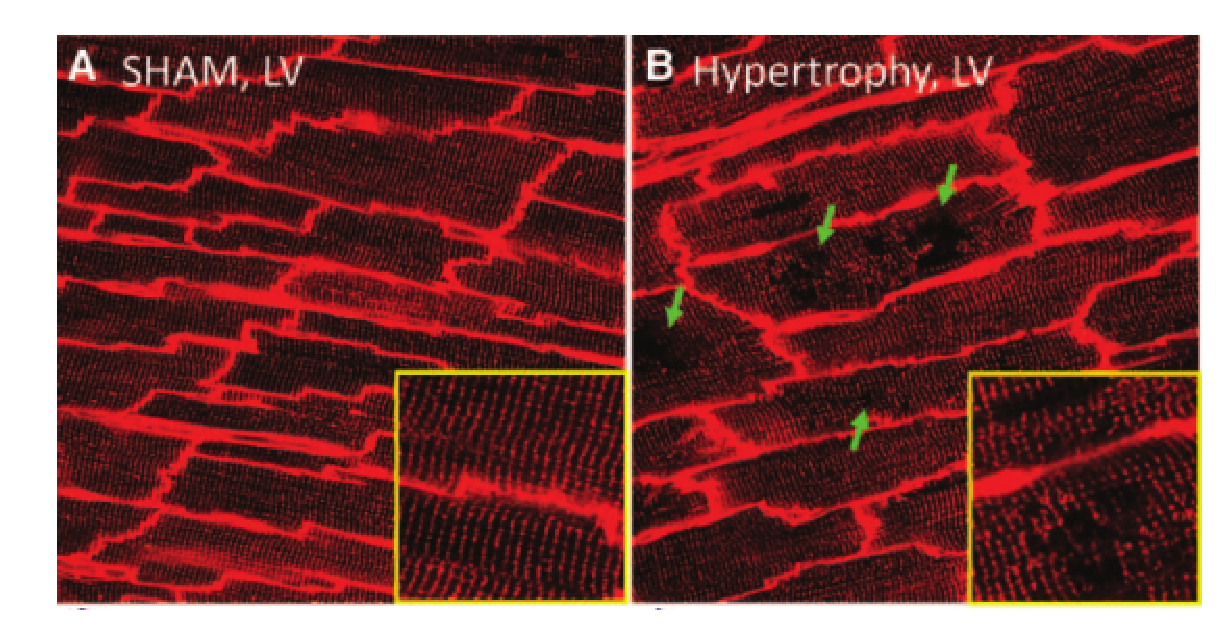
\includegraphics[height=5cm,
    angle=0]{./images/Ttubule_remodelling_Wei2010.eps}}
  \caption{Progressive T-tubule remodelling of LV myocyte in (A) hypertrophy
  and (B) early HF}
  \label{fig:Ttubule_remodelingWei2010}
\end{figure}


\begin{framed}
The molecular mechanism of T-tubule remodelling can be explained by the
downregulation in junctophilin-2 (JP-2) \ref{sec:JP-2}. 
\end{framed}

L-type $\Ca$ chanels (LCCs) are found 3-9 times more concentration in T-tubule
than in sarcolemma. The LCC on the surface is also co-localize with junctional
SR \citep{brette2003}, Fig.\ref{fig:Ttubule_scheme}. About 87\% of $I_\ca$ is
lost after detubulation.

The distribution of NCX is more controversal. Early studies showed that NCX is
predominant in T-tubule in guinea pig ventricular myocyte \citep{28}. Other
studies showed a more even distribution between T-tubule and sarcolemma
\citep{25,29}. In rat ventricular myocytes, NCX is found dominantly in T-tubule
\citep{26}. Almost all NCX activity are lost after detubulation in rat
ventricular myocytes.

\begin{figure}[hbt]
  \centerline{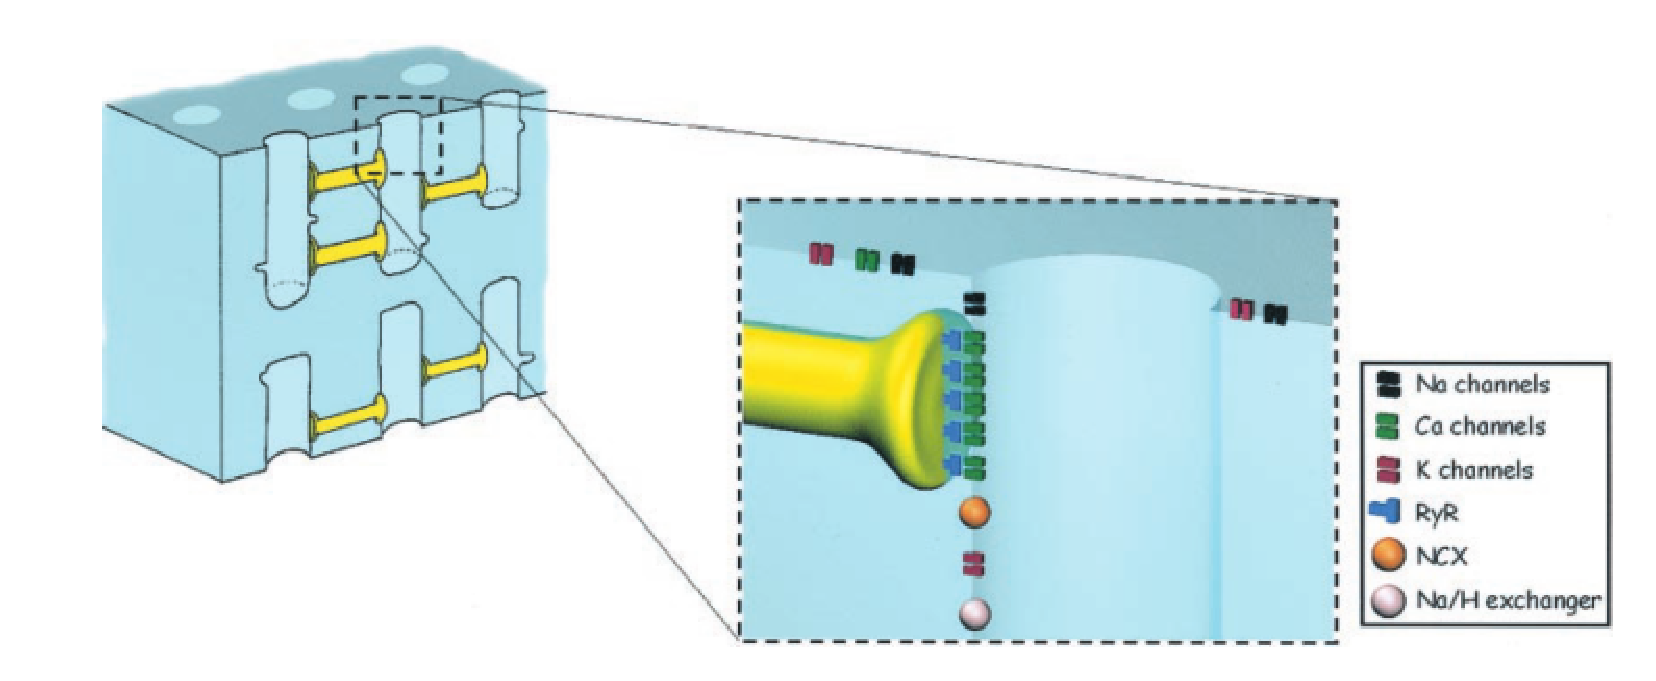
\includegraphics[height=5cm,
    angle=0]{./images/Ttubule_scheme.eps}}
  \caption{Protien distribution between T-tubule and external surface
  \citep{brette2003}}
  \label{fig:Ttubule_scheme}
\end{figure}

Na-H exchanger (regulate pH of the cell by extruding proton) is found with
higher concentration at the T-tubules and intercalated discs \citep{30}. 

Na channels were found localized to T-tubule in ventricular myocytes \citep{26}.
However, with different $\Na$ isoforms, the distributions of them are
different. Cardiac Na$_v$ 1.5 is found majority in intercalated disc, while
brain isoforms Na$_v$1.1, Na$_v$1.3 and Na$_v$1.6 are found in T-tubule.
However, the functions of 'brain' isoforms are unknown in cardiac
\citep{brette2003}. $I_\na$ shows uniform distribution between T-tubule and
surface membrane, similarly to $I_\k, I_\to, I_\text{K1}$ (even though the
proteins that underline channel are located predominantly on T-tubule. So,
there are controversies here). Nevertheless, TASK-1 $I_\text{Kss}$ showed to
concentrate at T-tubule.

Early studies showed K channels (Kv1.2, Kv4.2, Kv1.5 and Kv2.1) concentrate at
the surface membrane of rat ventricular myocytes, with highest density at the
intercalated discs \citep{33}. However, in later study, Kv4.2, the one that
underline $I_\to$ was showed to be localized predominantly to the T-tubular
system; and similarly to the case of TASK-1 (underline steady-state outward
current $I_\text{ss}$) and Kir2.1 (underline inward rectifier current
$I_\text{K1}$.


In mouse, heart rate is 300-400 bpm (i.e. 5-7 beats/sec). In pig, the heart rate
is $<100$ bpm.



\section{Hoang-Trong (201x)}

\citep{pogwizd2001} showed that reduced background $\K$ current ($I_{K1}$) and
increased NCX currents can act synergistically such that a spontaneous cell-wide
release of $\Ca$ will lead to a larger membrane depolarization, and thus be
potentially more arrhythmogenic than an equivalent $\Ca$ release in a healthy
cell. This can be tested with our model.




%%% Local Variables: 
%%% mode: latex
%%% TeX-master: "mainfile"
%%% End: 
